\documentclass[article,12pt]{elsarticle}
\usepackage[utf8]{inputenc}
\usepackage{graphicx}
\usepackage{booktabs}
\usepackage{subcaption}
\usepackage{amssymb}
\usepackage{flushend}
\usepackage{float}
\usepackage{amsmath}
\usepackage{amsfonts}
\usepackage{dcolumn}
\usepackage{amsthm}
\usepackage{caption}
\usepackage{lmodern}
\usepackage{booktabs}
\usepackage{color}
\usepackage{longtable}
\usepackage{rotating}
\usepackage{etoolbox}
\usepackage{hyperref}
\usepackage{comment}
\usepackage{pdflscape}
\usepackage{comment}
\usepackage[table,xcdraw]{xcolor}
\usepackage[framemethod=TikZ]{mdframed}
\usepackage[a4paper, left=1.5cm, right=1.5cm, top=2cm, bottom=2cm]{geometry}

\begin{document}

\mdfsetup{innertopmargin=10pt,linecolor=blue!20,%
linewidth=2pt,topline=true,
frametitleaboveskip=\dimexpr-\ht\strutbox\relax,}

\begin{frontmatter}
    \title{Laboratorio de Óptica \\ Práctica VIII: Interferencia y Difracción}
    \author{López González Andrés$^1$, Reyes Saldivar Ailton Uriel$^2$ y Gante Morales Pedro José$^3$}
    \address{$^1$ Facultad de Ciencias, Universidad Nacional Autónoma de México, México CDMX.}

\begin{abstract}
En esta práctica se estudiaron los fenómenos de interferencia y difracción utilizando láseres monocromáticos y sistemas de rendijas simples y dobles. A partir del patrón de interferencia de Young, se determinaron experimentalmente separaciones entre rendijas de $a = 0.0997 \pm 0.007\, \text{mm}$ y $a = 0.16 \pm 0.016\, \text{mm}$, mientras que la longitud de onda de un láser desconocido se estimó en $ \lambda = 399.83 \pm 0.58\, \text{nm}$ y $404.32 \pm 0.59\, \text{nm}$. En el experimento de difracción con rendija simple, se obtuvo un ancho promedio de rendija de $b = 0.20 \pm 0.02\, \text{mm}$, con el cual se calculó una longitud de onda de $\lambda = 523.2 \pm 8\, \text{nm}$ para un segundo láser. Los resultados obtenidos son consistentes con los valores esperados para láseres visibles, confirmando la validez de los modelos teóricos.

\end{abstract}
    
\end{frontmatter}

\section{Introducción}

\section*{Introducción}

El estudio de la luz y sus propiedades ha llevado a algunos de los descubrimientos más fundamentales en la física, siendo los fenómenos de interferencia y difracción dos de las manifestaciones más destacadas del carácter ondulatorio de la radiación electromagnética. Estas propiedades no solo permiten evidenciar la naturaleza de la luz más allá de su comportamiento corpuscular, sino que también constituyen herramientas esenciales para el análisis de estructuras microscópicas y nanométricas, con aplicaciones que abarcan desde la caracterización de materiales hasta la observación de estructuras biológicas como el ADN \cite{hecht2000optica, pedrotti2018optics, barrios2025interferencia}.

\subsection*{Interferencia de dos ondas}

Consideremos dos ondas planas, $\vec{E}_1$ y $\vec{E}_2$, que poseen la misma frecuencia y llegan a un punto $P$:

\begin{equation}
\vec{E}_1 = \vec{E}_{01} \cos(ks_1 - \omega t + \phi_1) \label{eq1}
\end{equation}
\cite{barrios2025interferencia}

\begin{equation}
\vec{E}_2 = \vec{E}_{02} \cos(ks_2 - \omega t + \phi_2) \label{eq2}
\end{equation}
\cite{barrios2025interferencia}

Donde $k = \frac{2\pi}{\lambda}$, $s_1$ y $s_2$ son las distancias recorridas por cada onda, $\phi_1$ y $\phi_2$ son las fases iniciales, y $\vec{E}_{01}$, $\vec{E}_{02}$ son las amplitudes. La superposición de estas ondas genera un campo neto en el punto $P$:

\begin{equation}
\vec{E}_P = \vec{E}_1 + \vec{E}_2 \label{eq3}
\end{equation}
\cite{barrios2025interferencia}

Dado que lo que se mide experimentalmente es la irradiancia (energía por unidad de área), esta se define como:

\begin{equation}
I = \varepsilon_0 c \langle \vec{E} \cdot \vec{E} \rangle \label{eq4}
\end{equation}
\cite{griffiths1999electrodynamics, barrios2025interferencia}

Para el caso de la superposición de dos ondas, la irradiancia total se expande en tres términos: dos individuales y uno de interferencia:

\begin{equation}
I = I_1 + I_2 + I_{12} \quad \text{con} \quad I_{12} = 2\varepsilon_0 c \langle \vec{E}_1 \cdot \vec{E}_2 \rangle \label{eq6}
\end{equation}
\cite{barrios2025interferencia}

Este término contiene la información sobre la diferencia de fase total entre las ondas:

\begin{equation}
I_{12} = \varepsilon_0 c (\vec{E}_{01} \cdot \vec{E}_{02}) \langle \cos \delta \rangle \quad \text{con} \quad \delta = k(s_2 - s_1) + \phi_2 - \phi_1 \label{eq7}
\end{equation}
\cite{barrios2025interferencia}

Si ambas ondas tienen polarización paralela y se asume que provienen de la misma fuente, el término de interferencia puede simplificarse a:

\begin{equation}
I_{12} = 2\sqrt{I_1 I_2} \langle \cos \delta \rangle \label{eq10}
\end{equation}
\cite{barrios2025interferencia}

\subsection*{Condiciones de interferencia: coherencia}

Cuando las fuentes no mantienen una relación constante de fase, se dice que son incoherentes. En ese caso, la expresión del término de interferencia se convierte en:

\begin{equation}
I_{12} = 2\sqrt{I_1 I_2} \langle \cos \delta(t) \rangle \label{eq11}
\end{equation}
\cite{barrios2025interferencia}

Si la variación de fase es aleatoria y suficientemente rápida, el promedio temporal tiende a cero y se obtiene simplemente:

\begin{equation}
I = I_1 + I_2 \label{eq12}
\end{equation}
\cite{barrios2025interferencia}

En contraste, cuando las ondas son coherentes (misma fuente, misma frecuencia y fase estable), se mantiene la relación de interferencia:

\begin{equation}
I = I_1 + I_2 + 2\sqrt{I_1 I_2} \cos \delta \label{eq13}
\end{equation}
\cite{barrios2025interferencia}

Cuando la diferencia de fase es un múltiplo entero de $2\pi$, se produce interferencia constructiva:

\begin{equation}
I_{\text{max}} = I_1 + I_2 + 2\sqrt{I_1 I_2} \label{eq14}
\end{equation}
\cite{barrios2025interferencia}

En cambio, si la diferencia de fase es un múltiplo impar de $\pi$, se da la interferencia destructiva:

\begin{equation}
I_{\text{min}} = I_1 + I_2 - 2\sqrt{I_1 I_2} \label{eq15}
\end{equation}
\cite{barrios2025interferencia}

\subsection*{Interferencia en doble rendija}

El experimento de la doble rendija de Young es uno de los ejemplos más clásicos para ilustrar interferencia. En este caso, las rendijas están separadas por una distancia $a$ y la pantalla se encuentra a una distancia $L$ del orden de varios centímetros o metros. La diferencia de caminos es:

\begin{equation}
\Delta = a \sin \theta \label{eq18}
\end{equation}
\cite{hecht2000optica, barrios2025interferencia}

Bajo la aproximación de ángulo pequeño ($\sin \theta \approx \tan \theta \approx y/L$), la distribución de intensidad sobre la pantalla es:

\begin{equation}
I = 4I_0 \cos^2 \left( \frac{\pi a y}{\lambda L} \right) \label{eq21}
\end{equation}
\cite{barrios2025interferencia}

Los máximos de interferencia (franjas brillantes) se encuentran en:

\begin{equation}
y_{\text{max}} = \frac{m \lambda L}{a}, \quad m = 0, \pm1, \pm2, \ldots \label{eq22}
\end{equation}
\cite{barrios2025interferencia}

Y los mínimos (franjas oscuras) en:

\begin{equation}
y_{\text{min}, m} = \frac{\lambda L}{a} \left(m \pm \frac{1}{2} \right) \label{eq23}
\end{equation}
\cite{barrios2025interferencia}

\subsection*{Difracción por una rendija}

La difracción ocurre incluso con una sola rendija debido al ancho finito de la abertura. En el régimen de Fraunhofer, el patrón de difracción se modela por la siguiente función:

\begin{equation}
I = I_0 \left( \frac{\sin \beta}{\beta} \right)^2, \quad \beta = \frac{\pi b \sin \theta}{\lambda} \label{eq24}
\end{equation}
\cite{pedrotti2018optics, barrios2025interferencia}

Utilizando la misma aproximación de ángulo pequeño, la posición de los mínimos se calcula como:

\begin{equation}
y_{\text{min}, m} = \frac{m \lambda L}{b}, \quad m = \pm1, \pm2, \ldots \label{eq26}
\end{equation}
\cite{barrios2025interferencia}

\subsection*{Superposición de interferencia y difracción}

En el experimento de la doble rendija, el patrón observado es en realidad una superposición del patrón de interferencia modulado por la envolvente de difracción. La expresión completa para la irradiancia en este caso es:

\begin{equation}
I(y) = 4I_0 \left( \frac{\sin \left( \frac{\pi b y}{\lambda L} \right)}{\left( \frac{\pi b y}{\lambda L} \right)} \right)^2 \cos^2 \left( \frac{\pi a y}{\lambda L} \right) \label{eq27}
\end{equation}
\cite{barrios2025interferencia}

Este comportamiento complejo permite, mediante el análisis del patrón, determinar parámetros como el ancho de la rendija, la separación entre rendijas o incluso la longitud de onda de la luz utilizada, siendo de gran utilidad en aplicaciones prácticas de metrología óptica \cite{hecht2000optica, barrios2025interferencia}.



\subsection{Hipótesis}
Si se proyecta un haz láser monocromático sobre una o dos rendijas delgadas, entonces se observará un patrón de franjas oscuras y brillantes en una pantalla, debido a los fenómenos de interferencia y difracción. A partir de dicho patrón, es posible calcular experimentalmente parámetros como la separación entre rendijas, el ancho de las rendijas o la longitud de onda de la luz utilizada, siempre que se mantenga la coherencia del haz y se tomen adecuadamente las medidas de distancia y posición.

\subsection{Objetivos}
\begin{itemize}
    \item Estudiar el patrón de interferencia producido por una doble rendija iluminada con un láser monocromático.
    \item Determinar la separación entre rendijas a partir de la posición de las franjas de interferencia destructiva.
    \item Calcular la longitud de onda de una fuente láser desconocida utilizando un patrón de interferencia con parámetros previamente medidos.
    \item Analizar el patrón de difracción generado por una rendija simple e identificar las posiciones de los mínimos de irradiancia.
    \item Determinar el ancho de una rendija mediante el patrón de difracción y, posteriormente, calcular la longitud de onda de un láser desconocido a partir de dicho patrón.
    \item Comparar los valores experimentales con los datos teóricos esperados para evaluar la precisión del montaje óptico.
\end{itemize}

\section{Desarrollo Experimental}



\subsection*{Doble rendija de Young}

Un experimento famoso es el de la doble rendija de Young, el cual utiliza dos rendijas muy cercanas que simulan dos fuentes de luz coherentes. Estas producen interferencia constructiva y destructiva en una pantalla de observación. A partir del patrón de interferencia generado, es posible determinar tanto la separación entre las rendijas como la longitud de onda de la luz empleada. Una de las expresiones que describe este fenómeno es:

\begin{equation}
y_{\text{min}, m} = \frac{\lambda L}{a} \left( m \pm \frac{1}{2} \right)
\end{equation}

Una característica importante del patrón de interferencia de Young es que, al estar compuesto por dos rendijas, presenta además un patrón de difracción que modula el patrón de interferencia. Este patrón de difracción contiene información sobre el ancho de cada rendija, pero en este experimento nos enfocaremos en el análisis del patrón de doble rendija. 

De la teoría de interferencia se puede deducir una relación entre la posición de las franjas de interferencia destructiva, la longitud de onda, la distancia $L$ entre las rendijas y la pantalla, la separación entre rendijas $a$, y el orden de interferencia $m$. Es importante notar que todas las posiciones se miden con respecto al centro del patrón.

Este experimento constará de dos partes. En la primera, se utilizará el patrón de interferencia destructiva para encontrar la separación entre rendijas mediante la ecuación:

\begin{equation}
a = \frac{\lambda L}{y_{\text{min}, m}} \left( m \pm \frac{1}{2} \right)
\end{equation}

En la segunda parte, se determinará la longitud de onda de un láser desconocido con la expresión:

\begin{equation}
\lambda = \frac{a \, y_{\text{min}, m}}{L \left( m \pm \frac{1}{2} \right)}
\end{equation}

Para la primera parte, el arreglo experimental consiste en un láser de $\lambda=650nm$, una diapositiva con dos rendijas muy cercanas y una pantalla de proyección. Las rendijas se deben colocar próximas al láser de forma que ambas sean iluminadas homogéneamente. La pantalla se sitúa a una distancia $L$ y en ella se observará el patrón de interferencia. El patrón de Young será el que presenta lóbulos más pequeños.

Para identificar el centro del patrón, es recomendable retirar momentáneamente la diapositiva con las rendijas y marcar la posición en que incide directamente el haz láser. Luego, se colocan nuevamente las rendijas y se marcan con lápiz las posiciones centrales de las franjas oscuras (interferencia destructiva), ya que estas son más fáciles de identificar visualmente.

Para una correcta visualización del patrón, se recomienda realizar las marcas en ausencia de luz ambiental. Posteriormente, con la luz encendida y con ayuda de un vernier, se miden las distancias desde cada marca hasta el centro del patrón. Con estos datos, se construye una tabla con la distancia de la franja oscura, la distancia a la pantalla $L$, la longitud de onda y el orden de interferencia. Al despejar $a$ en la ecuación correspondiente y aplicarla a todos los datos, se obtiene una estimación de la separación de las rendijas.

En este experimento se utilizaron dos pares de rendijas: la primera con una separación teórica de $0.10\, \text{mm}$ y la segunda de $0.16\, \text{mm}$. Para cada una, se midió la distancia $a$ de forma experimental siguiendo el procedimiento descrito.

Para la segunda parte, utilizando la separación entre rendijas medida anteriormente, se despeja la ecuación para calcular la longitud de onda del láser:

\[
\lambda = \frac{a \, y_{\text{min}, m}}{L \left( m \pm \frac{1}{2} \right)}
\]

En el arreglo experimental, simplemente se sustituye el láser rojo por otro de diferente color, cuya longitud de onda se desconoce. Se repite el procedimiento de marcado y medición para las franjas oscuras. Con los datos obtenidos se construye una tabla, a partir de la cual se calcula una longitud de onda promedio para cada par de rendijas.

\subsection*{Patrón de difracción}

La teoría predice la creación de un patrón de franjas de interferencia constructiva y destructiva, cuya distribución depende del tamaño de la abertura $b$, la longitud de onda $\lambda$ de la luz incidente y el orden de interferencia $m$. En la primera parte de este experimento se determinará el tamaño de una rendija a partir de la medición del patrón de difracción.

Para ello, se utiliza un láser y una pantalla de observación colocada a una distancia $L$ de la rendija. El láser debe incidir de forma que su sección transversal ilumine completamente la abertura. Al hacerlo, se genera un patrón de difracción sobre la pantalla. Dado que estos patrones suelen ser tenues, es fundamental trabajar en condiciones de baja iluminación.

En la pantalla se marcan, con lápiz, las posiciones centrales de las franjas oscuras (interferencia destructiva), así como el centro del patrón. Con la luz encendida, y utilizando un vernier, se miden las distancias desde las marcas hasta el centro. También se registra el orden $m$ correspondiente a cada franja.

Con estos datos, se construye una tabla con las posiciones $y$, el orden $m$, la distancia $L$ y la longitud de onda conocida. Para cada conjunto de datos se calcula el ancho de la rendija usando:

\begin{equation}
b = \frac{m \lambda L}{y}
\end{equation}

Posteriormente, se obtiene el tamaño promedio de la rendija, junto con su incertidumbre absoluta.

En la segunda parte del experimento, se usará la información del tamaño de la rendija para calcular la longitud de onda de un láser de otro color. Para esto se emplea la ecuación:

\begin{equation}
\lambda = \frac{b \, y}{mL}
\end{equation}

El procedimiento es el mismo que en la primera parte: se registra la posición de las franjas oscuras, el orden de interferencia $m$, el ancho $b$ de la rendija y la distancia $L$ a la pantalla. Para cada caso se calcula la longitud de onda, y finalmente se promedian todos los valores. La incertidumbre se obtiene mediante propagación de errores, sumando en cuadratura la incertidumbre teórica con la incertidumbre estadística.


\begin{figure}[H]
    \centering
    \begin{subfigure}[b]{0.2\textwidth}
        \centering
        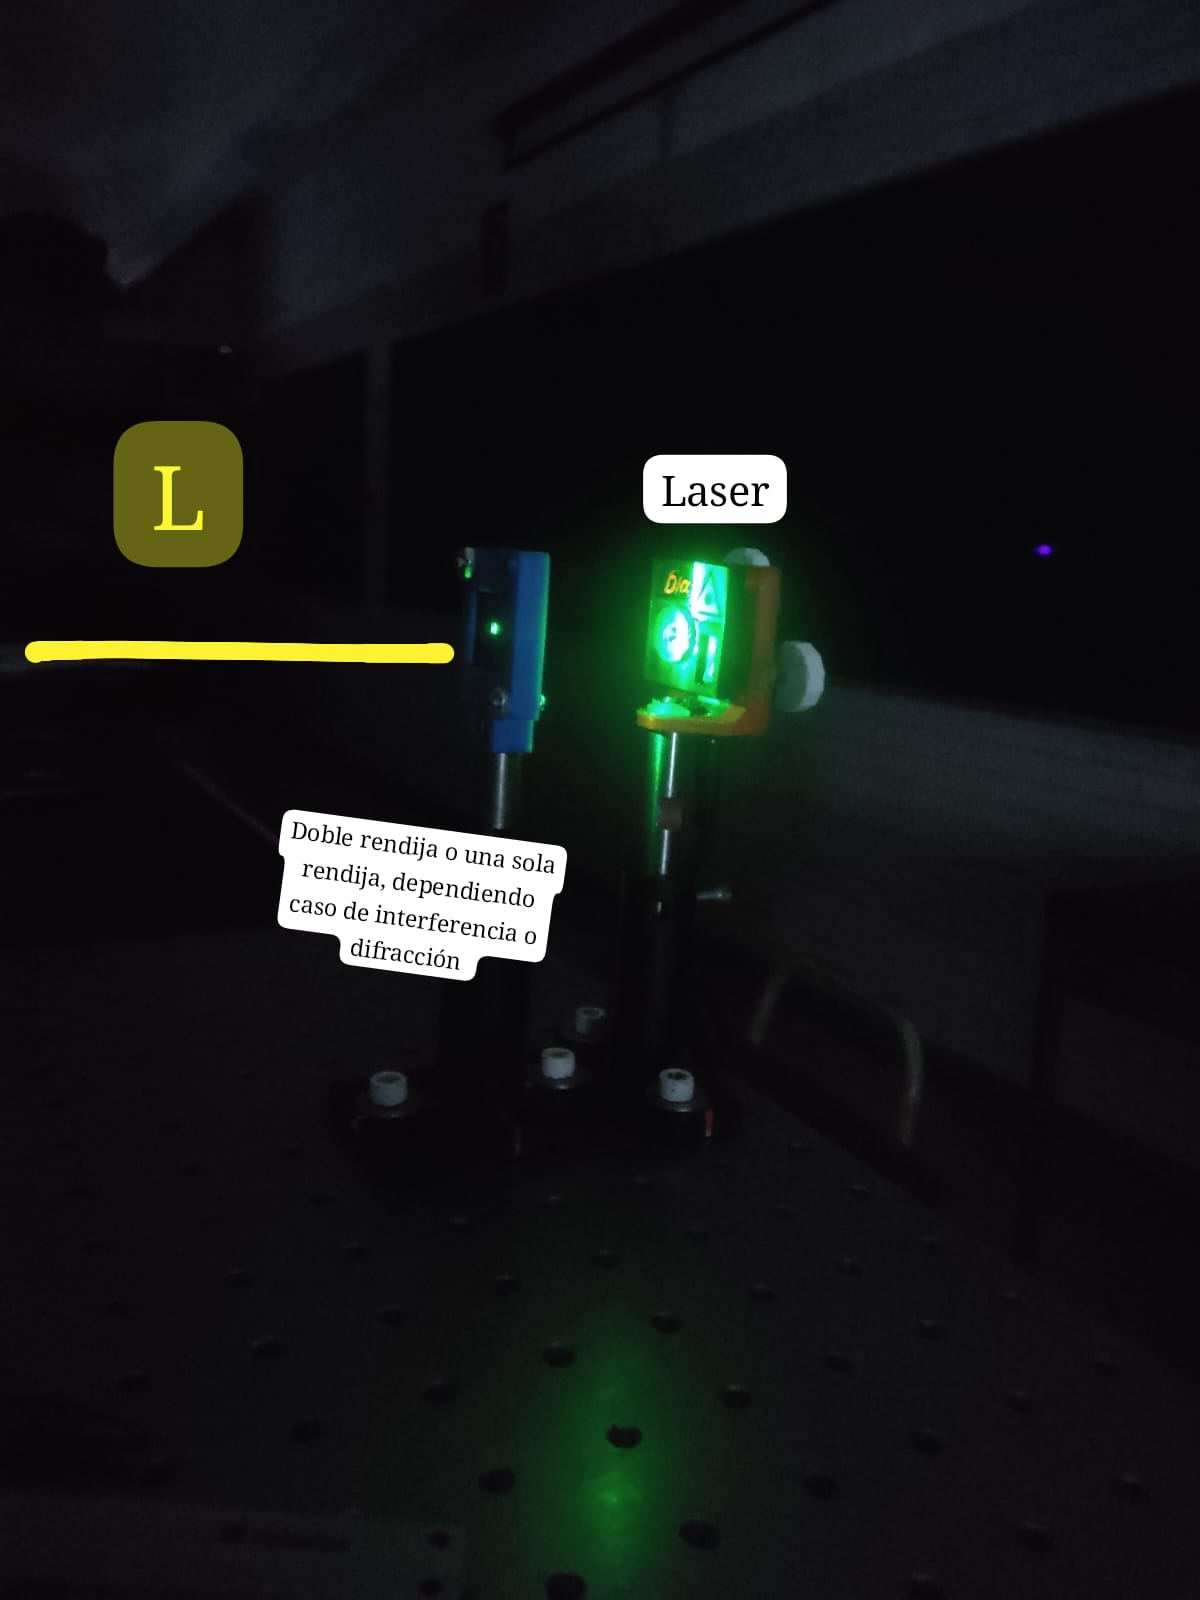
\includegraphics[width=\textwidth]{1.jpeg}
        \caption*{}
        \label{fig:imagen1}
    \end{subfigure}
    \hspace{1cm} % Espacio horizontal entre las dos imágenes
    \begin{subfigure}[b]{0.2\textwidth}
        \centering
        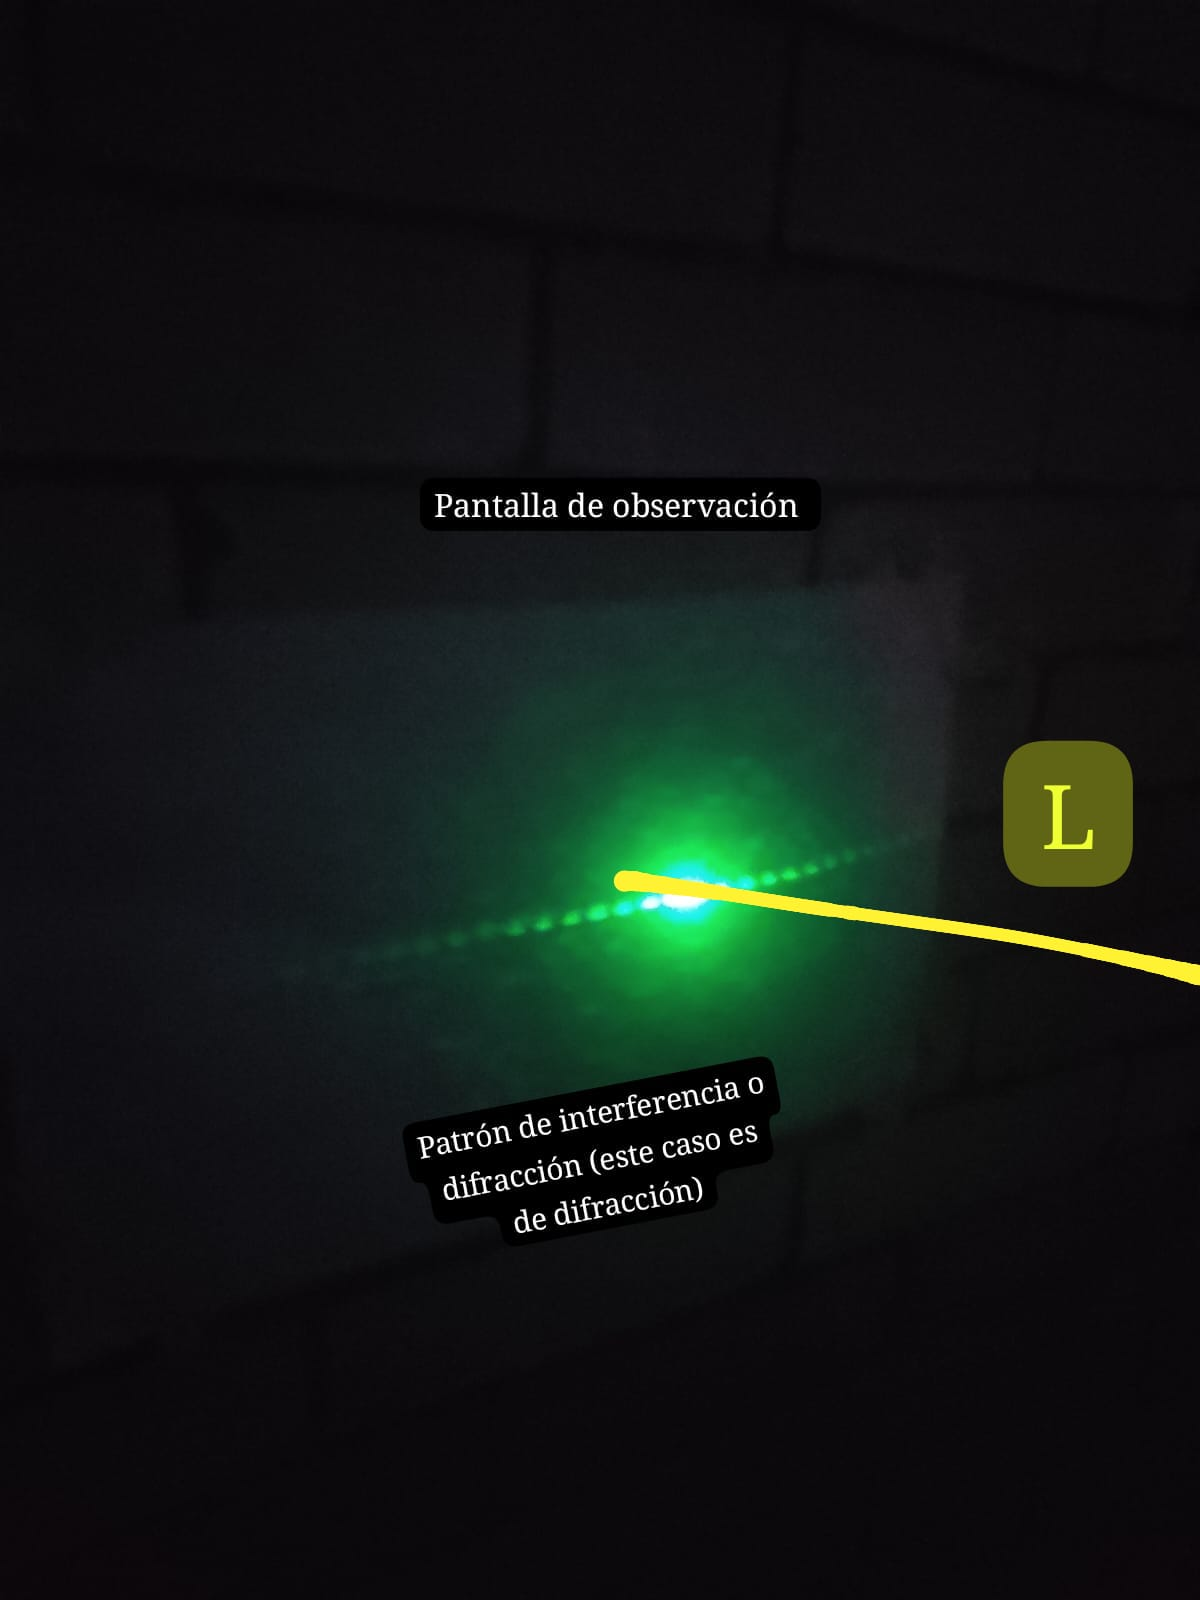
\includegraphics[width=\textwidth]{2.jpeg}
        \caption*{}
        \label{fig:imagen2}
    \end{subfigure}
    \caption{Arreglo general para los 2 experimentos (Young y Difracción)}
    \label{fig:comparacion}
\end{figure}




\section{Resultados y tratamiento de datos}

A continuación se muestran las tablas con los resultados obtenidos, para visualizar con más cuidado la tabla ásí como los cáculos pueden dirigirse al excel original. \cite{Excel}
\subsection{DOBLE RENDIJA}

\begin{table}[H]
\centering
\resizebox{\textwidth}{!}{%
\rowcolors{2}{green!20}{white}
\begin{tabular}{|c|c|c|c|c|c|c|c|c|c|c|}
\hline
\rowcolor{green!40}
$\lambda$ [nm] & $L$ [cm] & $\Delta L$ [cm] & $y$ [mm] & $\Delta y$ [mm] & $m$ & $a$ [mm] & $\sigma_{\text{nom}}$ [mm] & $\sigma_{\text{est}}$ [mm] & Promedio [mm] & $\Delta a$ [mm] \\
\hline
650.00 & 390.4 & 0.5 & 39.30 & 0.01 & 2.00 & 0.16 & 0.0002 & 0.016 & 0.16 & 0.16 \\
650.00 & 390.4 & 0.5 & 22.98 & 0.01 & 1.00 & 0.1656397 & & & & \\
650.00 & 390.4 & 0.5 & 6.48 & 0.01 & 0.50 & 0.1958025 & & & & \\
650.00 & 390.4 & 0.5 & -9.12 & 0.01 & -0.50 & 0.2391228 & & & & \\
650.00 & 390.4 & 0.5 & -26.99 & 0.01 & -1.00 & 0.1410300 & & & & \\
650.00 & 390.4 & 0.5 & -41.63 & 0.01 & -2.00 & 0.1523901 & & & & \\
\hline
\end{tabular}%
}
\caption{Deducción de la separación \( a \) entre rendijas (para el par de rendijas $a=0.16mm$).}
\end{table}

\begin{table}[H]
\centering
\resizebox{\textwidth}{!}{%
\rowcolors{2}{orange!10}{white}
\begin{tabular}{|c|c|c|c|c|c|c|c|c|c|c|c|}
\hline
\rowcolor{orange!30}
$a$ [mm] & $\Delta a$ [mm] & $L$ [cm] & $\Delta L$ [cm] & $y$ [mm] & $\Delta y$ [mm] & $m$ & $\lambda$ [nm] & $\sigma_{\text{nom}}$ [mm] & $\sigma_{\text{est}}$ [mm] & Promedio [nm] & $\Delta \lambda$ [nm] \\
\hline
0.1592 & 0.01 & 390.4 & 0.5 & 33.72 & 0.01 & 3.00 & 392.96 & 0.000004 & 0.583 & 399.83 & 0.5834 \\
0.1592 & 0.01 & 390.4 & 0.5 & 24.64 & 0.01 & 2.00 & 402.00 & & & & \\
0.1592 & 0.01 & 390.4 & 0.5 & 15.08 & 0.01 & 1.00 & 410.05 & & & & \\
0.1592 & 0.01 & 390.4 & 0.5 & 4.96  & 0.01 & 0.00 & 404.61 & & & & \\
0.1592 & 0.01 & 390.4 & 0.5 & -4.67 & 0.01 & 0.00 & 380.96 & & & & \\
0.1592 & 0.01 & 390.4 & 0.5 & -14.41 & 0.01 & -1.00 & 391.83 & & & & \\
0.1592 & 0.01 & 390.4 & 0.5 & -24.35 & 0.01 & -2.00 & 397.27 & & & & \\
0.1592 & 0.01 & 390.4 & 0.5 & -35.95 & 0.01 & -3.00 & 418.95 & & & & \\
\hline
\end{tabular}%
}
\caption{Deducción de la longitud de onda \( \lambda \) a partir de una separación conocida \( a = 0.1592\,\text{mm} \), con cálculo de promedio y error.}
\end{table}



\begin{table}[H]
\centering
\resizebox{\textwidth}{!}{%
\rowcolors{2}{green!10}{white}
\begin{tabular}{|c|c|c|c|c|c|c|c|c|c|c|}
\hline
\rowcolor{green!30}
$\lambda$ [nm] & $L$ [cm] & $\Delta L$ [cm] & $y$ [mm] & $\Delta y$ [mm] & $m$ & $a$ [mm] & $\sigma_{\text{nom}}$ [mm] & $\sigma_{\text{est}}$ [mm] & Promedio [mm] & $\Delta a$ [mm] \\
\hline
650.00 & 390.4 & 0.5 & 59.08 & 0.01 & 2.00 & 0.1074 & 0.0002 & 0.0067 & 0.0997 & 0.007 \\
650.00 & 390.4 & 0.5 & 38.33 & 0.01 & 1.00 & 0.0993 & & & & \\
650.00 & 390.4 & 0.5 & 12.38 & 0.01 & 0.00 & 0.1025 & & & & \\
650.00 & 390.4 & 0.5 & -15.48 & 0.01 & 0.00 & 0.0819 & & & & \\
650.00 & 390.4 & 0.5 & -37.94 & 0.01 & -1.00 & 0.1003 & & & & \\
650.00 & 390.4 & 0.5 & -59.31 & 0.01 & -2.00 & 0.1069 & & & & \\
\hline
\end{tabular}%
}
\caption{Deducción de la separación \( a \) entre rendijas (para el par de rendijas $a=0.16mm$).}
\end{table}

\begin{table}[H]
\centering
\resizebox{\textwidth}{!}{%
\rowcolors{2}{blue!10}{white}
\begin{tabular}{|c|c|c|c|c|c|c|c|c|c|c|c|}
\hline
\rowcolor{blue!30}
$a$ [mm] & $\Delta a$ [mm] & $L$ [cm] & $\Delta L$ [cm] & $y$ [mm] & $\Delta y$ [mm] & $m$ & $\lambda$ [nm] & $\sigma_{\text{nom}}$ [mm] & $\sigma_{\text{est}}$ [mm] & Promedio [nm] & $\Delta \lambda$ [nm] \\
\hline
0.100 & 0.01 & 390.4 & 0.5 & 54.70 & 0.01 & 3.00 & 399.27 & 0.000004& 0.59 &  404.32& 0.59\\
0.100 & 0.01 & 390.4 & 0.5 & 37.58 & 0.01 & 2.00 & 384.03 & & & & \\
0.100 & 0.01 & 390.4 & 0.5 & 22.55 & 0.01 & 1.00 & 384.07 & & & & \\
0.100 & 0.01 & 390.4 & 0.5 & 7.67  & 0.01 & 0.50 & 391.90 & & & & \\
0.100 & 0.01 & 390.4 & 0.5 & -8.39 & 0.01 & -0.50 & 428.69 & & & & \\
0.100 & 0.01 & 390.4 & 0.5 & -24.31 & 0.01 & -1.00 & 414.04 & & & & \\
0.100 & 0.01 & 390.4 & 0.5 & -40.16 & 0.01 & -2.00 & 410.40 & & & & \\
0.100 & 0.01 & 390.4 & 0.5 & -57.83 & 0.01 & -3.00 & 422.12 & & & & \\
\hline
\end{tabular}%
}
\caption{Deducción de la longitud de onda \( \lambda \) a partir de la separación \( a \) (para el par de rendijas $a=0.1mm$)}
\end{table}

Para el calculo de las incertidumbres usamos las ecuaciones localizada en el anexo de este documento, en el cual vienen especificamente de que trata cada una.

Los resultados obtenidos en esta práctica permitieron verificar experimentalmente las relaciones teóricas que describen la interferencia y difracción de la luz. En el caso del experimento de la doble rendija, se logró determinar la separación entre rendijas con una buena precisión. Para el primer conjunto de datos, se obtuvo un valor de $a = 0.0997 \pm 0.007\, \text{mm}$, y para el segundo, $a = 0.16 \pm 0.016\, \text{mm}$, ambos cercanos a los valores teóricos esperados.

Posteriormente, utilizando estas separaciones, se logró estimar la longitud de onda de un láser desconocido. En el caso de $a = 0.1592\, \text{mm}$, se obtuvo $\lambda = 399.83 \pm 0.58\, \text{nm}$, mientras que para $a = 0.1\, \text{mm}$, el resultado fue $\lambda = 404.32 \pm 0.59\, \text{nm}$, valores que corresponden a luz visible en la región azul-violeta del espectro electromagnético.


\subsection{DIFRACCIÓN}

\begin{table}[H]
\centering
\resizebox{\textwidth}{!}{%
\rowcolors{2}{orange!20}{white}
\begin{tabular}{|c|c|c|c|c|c|c|c|c|c|c|}
\hline
\rowcolor{orange!40}
$\lambda$ [nm] & $L$ [cm] & $\Delta L$ [cm] & $y$ [mm] & $\Delta y$ [mm] & $m$ & $b$ [mm] & $b_\text{nom}$ [mm] & $\sigma_\text{est}$ [mm] & Promedio [mm] & $\Delta b$ [mm] \\
\hline
650 & 390.3 & 0.05 & 5.072 & 0.01 & 4 & 0.20 & 0.016  & 0.01  & 0.2 & 0.02 \\
650 & 390.3 & 0.05 & 3.816 & 0.01 & 3 & 0.20 &  &  &  &  \\
650 & 390.3 & 0.05 & 2.21 & 0.01 & 2 & 0.23 &  &  &  &  \\
650 & 390.3 & 0.05 & 1.27 & 0.01 & 1 & 0.20 &  &  &  &  \\
650 & 390.3 & 0.05 & -1.23 & 0.01 & -1 & 0.21 &  &  &  &  \\
650 & 390.3 & 0.05 & -2.514 & 0.01 & -2 & 0.20 &  &  &  &  \\
650 & 390.3 & 0.05 & -3.93 & 0.01 & -3 & 0.19 &  &  &  &  \\
650 & 390.3 & 0.05 & -5.138 & 0.01 & -4 & 0.20 &  &  &  &  \\
\hline
\end{tabular}%
}
\caption{Deducción del tamaño de rendija \( b \) a partir del patrón de difracción.}
\end{table}

\begin{table}[H]
\centering
\resizebox{\textwidth}{!}{%
\rowcolors{2}{green!20}{white}
\begin{tabular}{|c|c|c|c|c|c|c|c|c|c|c|c|}
\hline
\rowcolor{green!40}
$b$ [mm] & $\Delta b$ [mm] & $L$ [cm] & $\Delta L$ [mm] & $y$ [mm] & $\Delta y$ [mm] & $m$ & $\lambda$ [nm] & $\lambda_\text{nom}$ [nm] & $\sigma_\text{est}$ [nm] & Promedio [nm]& $\Delta \lambda$\\
\hline
0.204 &  & 390.3 & 0.05 & 39.01 & 0.01 & 4 & 509 & 0.0003 & 8 & 523.2 & 8\\
0.204 &  & 390.3 & 0.05 & 29.72 & 0.01 & 3 & 517 &  &  & & \\
0.204 &  & 390.3 & 0.05 & 19.95 & 0.01 & 2 & 520 &  &  & & \\
0.204 &  & 390.3 & 0.05 & 10.04 & 0.01 & 1 & 524 &  &  & & \\
0.204 &  & 390.3 & 0.05 & -10.27 & 0.01 & -1 & 536 &  &  & & \\
0.204 &  & 390.3 & 0.05 & -20.48 & 0.01 & -2 & 534 &  &  &  &\\
0.204 &  & 390.3 & 0.05 & -30.15 & 0.01 & -3 & 524 &  &  &  &\\
0.204 &  & 390.3 & 0.05 & -40.13 & 0.01 & -4 & 523 &  &  & & \\
\hline
\end{tabular}%
}
\caption{Deducción de la longitud de onda \( \lambda \) usando el patrón de interferencia.}
\end{table}
Para el calculo de las incertidumbres usamos las ecuaciones localizada en el anexo de este documento, en el cual vienen especificamente de que trata cada una.

En el experimento de difracción por una rendija, se obtuvo un valor promedio del ancho de rendija de $b = 0.20 \pm 0.02\, \text{mm}$ utilizando un láser rojo de $\lambda = 650\, \text{nm}$. Con este valor de $b$, se calculó la longitud de onda de un segundo láser desconocido, resultando en $\lambda = 523.2 \pm 8\, \text{nm}$, que corresponde a luz verde, como era de esperarse.

Los datos experimentales presentan buena consistencia con la teoría y muestran la utilidad de estos fenómenos para realizar mediciones ópticas precisas. Las pequeñas discrepancias observadas pueden atribuirse a errores sistemáticos en la medición de distancias y alineación del sistema óptico, los cuales podrían reducirse con un montaje más preciso y condiciones de iluminación controladas.


\section{Conclusiones}

La práctica permitió verificar experimentalmente los fenómenos de interferencia y difracción mediante la medición de patrones generados por rendijas simples y dobles. En la primera parte, se determinó la separación entre rendijas utilizando un láser de $\lambda = 650\, \text{nm}$, obteniéndose valores promedio de $a = 0.0997 \pm 0.007\, \text{mm}$ y $a = 0.160 \pm 0.016\, \text{mm}$, en buena concordancia con los valores teóricos proporcionados.

Utilizando estas separaciones, se estimó la longitud de onda de un láser desconocido. Para $a = 0.1592\, \text{mm}$ se obtuvo $\lambda = 399.83 \pm 0.58\, \text{nm}$, mientras que para $a = 0.100\, \text{mm}$ el resultado fue $\lambda = 404.32 \pm 0.59\, \text{nm}$, lo que sugiere que se trató de una fuente de luz en el rango azul-violeta del espectro.

En el caso del patrón de difracción por una rendija, se estimó el ancho de la rendija como $b = 0.200 \pm 0.020\, \text{mm}$ a partir de un láser rojo. Este valor se utilizó para calcular la longitud de onda de otro láser, obteniéndose $\lambda = 523.2 \pm 8\, \text{nm}$, correspondiente a luz verde.

Los resultados muestran buena coherencia con los modelos teóricos, confirmando la naturaleza ondulatoria de la luz y la utilidad de estos patrones como herramientas cuantitativas en óptica. Las pequeñas discrepancias pueden atribuirse a errores sistemáticos de alineación o medición, que podrían reducirse en futuras repeticiones con un montaje más preciso.


\begin{thebibliography}{9}
\bibitem{griffiths1999electrodynamics} D. J. Griffiths, \textit{Introduction to Electrodynamics}, 3\textsuperscript{a} ed., Prentice Hall, 1999.
\bibitem{hecht2000optica} E. Hecht, \textit{Óptica}, 3\textsuperscript{a} ed., Addison Wesley, 2000.
\bibitem{pedrotti2018optics} F. L. Pedrotti, L. M. Pedrotti, L. S. Pedrotti, \textit{Introduction to Optics}, 3\textsuperscript{a} ed., Cambridge University Press, 2018.
\bibitem{barrios2025interferencia} Erick Barrios Barocio; Roxette Ramírez Arvidez, \textit{Interferencia y Difracción}, Óptica v.2025.\href{https://tsikbal.github.io/P%C3%A1ginas/%C3%81reas/F%C3%ADsica/%C3%93ptica/Optica_Fisica/Difracci%C3%B3n%20e%20Interferencia.html}{Enlace al documento}
\bibitem{Excel} A. Reyes, S. TablaS de Interferencia y difracción, Archivo Excel. 2025. Disponible en: \href{https://docs.google.com/spreadsheets/d/1XihNQc4zVtCAMRpLWDN6WFEjftBAhXA2/edit?usp=sharing&ouid=112625838925660900694&rtpof=true&sd=true}{Enlace al documento}
\end{thebibliography}


\section*{Anexo}

Incertidumbre nominal de la separación entre las rendijas en el experimento de de Young. 

\begin{mdframed}
    \label{incertidumbre P.A}
    \begin{equation}
        \sigma_{a}= \sqrt{\left(\frac{\lambda L\Delta y_{min}}{y_{min}^2}(m\pm 1/2)\right)^{2}+\left(\frac{\lambda\Delta L}{y_{min}}(m\pm 1/2)\right)^2}
    \end{equation}
\end{mdframed}

Incertidumbre estadística de la separación entre las rendijas.
\begin{mdframed}
 \label{incertidumbre PPP}
 \begin{equation}
\sigma_{est_a}=\sqrt{\frac{\sum_{i=1}^{N}(a-\bar{a})^2}{N(N-1)}}
\end{equation}
\end{mdframed}

Incertidumbre nominal de la longitud de onda en el experimento de de Young. 
\begin{mdframed}
    \label{incertidumbre P.A}
    \begin{equation}
        \sigma_{\lambda}= \sqrt{\left(\frac{y_{min} \Delta a}{L(m\pm 1/2)}\right)^{2}+\left(\frac{y_{min}a\Delta L}{L^2(m\pm 1/2)}\right)^2}
    \end{equation}
\end{mdframed}

Incertidumbre estadística de la longitud de onda.
\begin{mdframed}
 \label{incertidumbre PPP}
 \begin{equation}
\sigma_{est_\lambda}=\sqrt{\frac{\sum_{i=1}^{N}(\lambda-\bar{\lambda})^2}{N(N-1)}}
\end{equation}
\end{mdframed}

Incertidumbre nominal del tamaño de la rendija $b$
\begin{mdframed}
    \label{incertidumbre P.A}
    \begin{equation}
        \sigma_b= \sqrt{\left(\frac{m\lambda \Delta L}{y}\right)^{2}+\left(\frac{m\lambda L\Delta y}{y^2}\right)^2}
    \end{equation}
\end{mdframed}

Incertidumbre nominal para la longitud de onda en el experimento de difracción.
\begin{mdframed}
    \label{incertidumbre P.A}
    \begin{equation}
        \sigma_\lambda= \sqrt{\left(\frac{b \Delta y}{mL}\right)^{2}+\left(\frac{y\Delta b}{mL}\right)^2+\left(\frac{yb\Delta L}{mL^2}\right)^2}
    \end{equation}
\end{mdframed}







\end{document}